\section{Quadratics}
\subsection{Intro to Solving Quadratics}
\begin{definition}[Standard Form]
	$$f(x) = ax^2 + bx + c$$
	$$f(x) = 0$$
	$$ax^2 + bx + c = 0$$
	\begin{itemize}
	\item $a, \, b$ and $c$ are known numbers (coefficients and constants).
	\item $a$ cannot be 0, if $a = 0$, the equation becomes linear.
	\end{itemize}
	\textbf{Note: }All we really do is just finding the $x$ intercepts.
\end{definition}
\subsubsection{Cases}
There are a total of 3 cases a quadratic can have.
	\begin{example}[2 x Intercepts]
		\hfill
		\begin{center}
		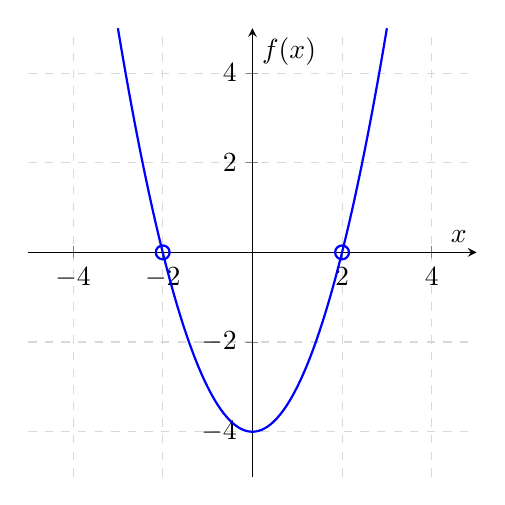
\begin{tikzpicture}
			\begin{axis}[
			    axis lines = center,
			    xlabel = $x$,
			    ylabel = $f(x)$,
			    xmin = -5, xmax = 5,
			    ymin = -5, ymax = 5,
			    grid = major,
			    grid style = {dashed, gray!30},
			    axis equal image
			]
			    \addplot [domain=-3:3, samples=100, thick, blue] {x^2 - 4};
				\draw[blue, thick] (axis cs:-2,0) circle(2.5pt);
				\draw[blue, thick] (axis cs:2,0) circle(2.5pt);
			\end{axis}
		\end{tikzpicture}
		\end{center}
		\begin{itemize}
			\item 2 Solutions.
			\item 2 Real Solutions.
			\item 2 Real $x$ Intercepts.
		\end{itemize}
	\end{example}
	\begin{example}[1 x Intercept]
		\hfill
		\begin{center}
		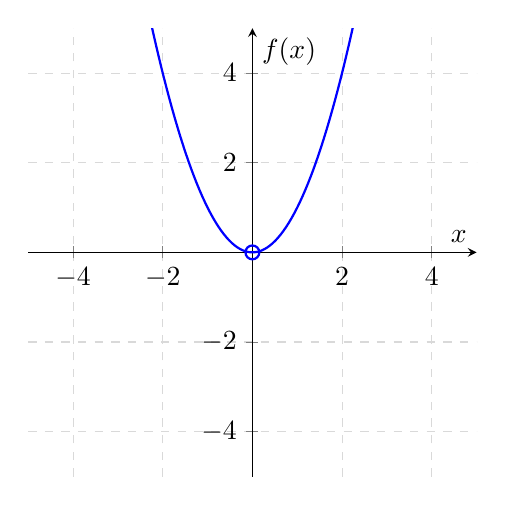
\begin{tikzpicture}
			\begin{axis}[
			    axis lines = center,
			    xlabel = $x$,
			    ylabel = $f(x)$,
			    xmin = -5, xmax = 5,
			    ymin = -5, ymax = 5,
			    grid = major,
			    grid style = {dashed, gray!30},
			    axis equal image
			]
			    \addplot [domain=-3:3, samples=100, thick, blue] {x^2};
				\draw[blue, thick] (axis cs:0,0) circle(2.5pt);
			\end{axis}
		\end{tikzpicture}
		\end{center}
		\begin{itemize}
			\item 1 Real Solutions.
			\item 1 Real $x$ Intercepts.
		\end{itemize}
	\end{example}
	\begin{example}[No x Intercept]
		\hfill
		\begin{center}
		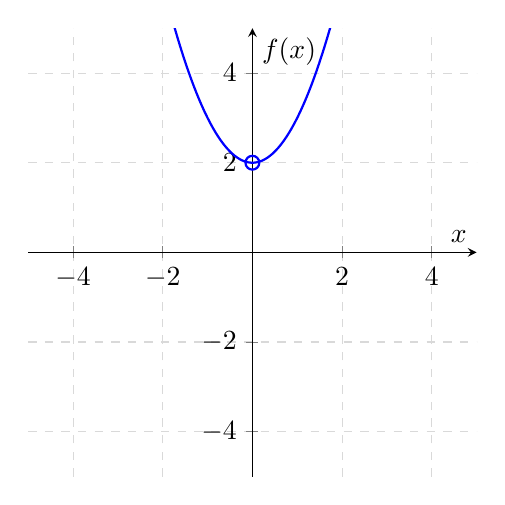
\begin{tikzpicture}
			\begin{axis}[
			    axis lines = center,
			    xlabel = $x$,
			    ylabel = $f(x)$,
			    xmin = -5, xmax = 5,
			    ymin = -5, ymax = 5,
			    grid = major,
			    grid style = {dashed, gray!30},
			    axis equal image
			]
			    \addplot [domain=-3:3, samples=100, thick, blue] {x^2 + 2};
				\draw[blue, thick] (axis cs:0,2) circle(2.5pt);
			\end{axis}
		\end{tikzpicture}
		\end{center}
		\begin{itemize}
			\item 2 Complex Solutions.
			\item No $x$ Intercepts.
		\end{itemize}
	\end{example}
